%! Author = danielmendes
%! Date = 26.01.25

\chapter{Views}\label{ch:views}
Im folgenden Kapitel werden die Performancevorteile von Sichten (engl.\ Views) in SQL betrachtet.
Zunächst wird auf virtuelle Sichten, ihre Vor- und Nachteile, das Verhalten bei Inserts sowie auf mögliche Szenarien eingegangen, in denen sie besonders vorteilhaft sein können.
Anschließend wird sich mit materialisierten Sichten beschäftigt, die physisch in der Datenbank gespeichert werden.
Zunächst wird eine Version mit Triggern implementiert, da MySQL keine native Unterstützung für materialisierte Sichten bietet, bevor die native Implementierung in PostgreSQL genutzt wird.
In den letzten beiden Kapiteln wird die Durchführung der Benchmarks näher betrachtet und die entstandenen Ergebnisse interpretiert.

\section{Virtuelle Views}\label{sec:virtuelle-views}

Grundlegend existieren Relationen, bzw.\ Tabellen, die durch das \texttt{CREATE TABLE}-Statement definiert werden, physisch in der Datenbank.
Damit sind sie persistent, was bedeutet, dass sie dauerhaft existieren und sich nicht ändern, es sei denn, sie werden explizit durch eine SQL-Änderungsanweisung dazu aufgefordert.
Dies entspricht der Dauerhaftigkeit des ACID-Prinzips (\cite{acid_eigenschaften}), die sicherstellt, dass bestätigte Transaktionen dauerhaft gespeichert bleiben und auch bei Systemausfällen nicht verloren gehen.
Es gibt jedoch eine weitere Klasse von SQL-Relationen, die nicht wie Tabellen physisch gespeichert werden (\cite[341--349, 353--366]{garcia2008database}).
%~\cite[S. 276--281]{schwartz2012high}
Sie werden als virtuelle Sichten bezeichnet.

\begin{quote}
    \enquote{A view is a table whose rows are not explicitly stored in the database but are computed as needed from a view definition.} (\cite[S. 86]{ramakrishnan2002database})
\end{quote}

Virtuelle Sichten werden durch einen Ausdruck definiert, der einer Abfrage ähnelt.
Sie können auch so abgefragt werden, als ob sie tatsächlich physisch existierten (vgl.\ \cite[S. 87]{ramakrishnan2002database}).
In einigen Fällen lassen sich sogar Datensätze über die Sicht ändern.

\vspace{-5pt}
\begin{lstlisting}[language=SQL,caption=Allgemeine View-Deklaration,label={lst:create_view}]
CREATE VIEW <name> AS <view-definition>;
\end{lstlisting}
\vspace{-5pt}

In dem Codeblock~\ref{lst:create_view} wird die Struktur der Definition einer View gezeigt.
Als Nächstes muss die \texttt{view-definition} mit einer SQL-Abfrage ersetzt werden, die den Inhalt der virtuellen Sicht abbilden soll.
Um dieses Vorgehen mit einem Beispiel näher zu veranschaulichen, werden die Tabellen Kunden (\ref{lst:tools-create-table-kunde}) und Bestellung (\ref{lst:tools-create-table-bestellung}) genutzt.
Nun wollen wir, dass die beiden Tabellen über die \texttt{KUNDEN\_ID} in der Sicht zusammengefügt werden, da sie sowohl der Primärschlüssel in der Kundentabelle als auch der Fremdschlüssel in der Bestellung ist.
Um in die SQL-Abfrage noch etwas mehr Komplexität zu bringen, soll neben der Join-Operation auch der Umsatz pro Jahr und pro Stadt aggregiert werden.
Die View \texttt{KUNDEN\_OVERVIEW} hat folgende Struktur:

\vspace{-5pt}
\lstinputlisting[
    language=sql,
    caption=View Deklarierung,
    label={lst:create_kunden_bestellung_view},
    style=custom_daniel,
]{Scripts/Views/01_create_view.sql}

Diese Aggregation könnte beispielsweise von einem Marketingteam genutzt werden, um schwache Regionen pro Jahr zu identifizieren und gezielt in diesen nachzusteuern.
Wenn die Daten dieser virtuellen Sicht abgefragt werden sollen, wird der Name in der FROM-Klausel adressiert und es wird darauf vertraut, dass das Datenbankmanagementsystem die benötigten Tupel erzielt (siehe~\ref{lst:select-view}).
Dabei operiert das DBMS direkt auf den Relationen, die die virtuelle Sicht definieren.
In diesem Fall handelt es sich um die Kunden- und Bestelltabelle.

\vspace{-5pt}
\begin{lstlisting}[language=SQL,caption=SQL-Befehl mit verwendeter View,label={lst:select-view}]
SELECT * FROM KUNDEN_OVERVIEW
ORDER BY Jahr ASC, Gesamtumsatz DESC;
\end{lstlisting}
\vspace{-5pt}

Eine weitere Möglichkeit, die Funktionsweise einer Sicht besser zu verstehen, besteht darin, sie in einer FROM-Klausel durch eine Unterabfrage zu ersetzen, die identisch mit der Sichtdefinition ist.
Damit Bezug auf die Tupel genommen werden kann, muss die Unterabfrage noch mit einer Tupelvariablen ergänzt werden.
Die SQL-Abfrage aus~\ref{lst:select-without-view} liefert das gleiche Ergebnis wie die aus~\ref{lst:select-view}, wenn die View wie im Beispiel~\ref{lst:create_kunden_bestellung_view} definiert wird.
Zu dem Einfluss auf die Performance wird im Unterkapitel~\ref{sec:durchfuhrung-der-benchmarks} eingegangen.

\lstinputlisting[
    language=sql,
    caption=Select-Befehl ohne Sicht,
    label={lst:select-without-view},
    style=custom_daniel,
]{Scripts/Views/02_select_without_view.sql}

Man kann den Attributen einer Sicht auch eigene Namen vergeben, indem man sie in Klammern hinter dem Namen der Sicht aus der \texttt{CREATE VIEW}-Anweisung auflistet.
Die Definition einer Sicht kann mit \texttt{DROP VIEW <view-name>} gelöscht werden, wodurch keine Abfragen mehr auf dieser Sicht ausgeführt werden können.
Das Löschen der Sicht hat jedoch keine Auswirkungen auf die Tupel der zugrundeliegenden Tabellen.
Im Gegensatz dazu würde \texttt{DROP TABLE <table-name>} die Tabelle löschen und damit auch die darauf basierenden Sichten unbrauchbar machen, da ihre Definitionen auf der gelöschten Tabelle beruhen.

Abgesehen vom Löschen der Tabellen kann man auch Einfügungen an der View durchführen.
Dies ist aber nicht uneingeschränkt möglich und nur unter bestimmten Bedingungen erlaubt.
Zum einen muss die Sicht durch eine einfache Abfrage aus nur einer einzigen Relation definiert sein.
Zum anderen muss die \texttt{SELECT}-Klausel ausreichend Attribute umfassen, sodass fehlende Werte bei Einfügungen mit \texttt{NULL} oder anderen definierten Standardwerten ergänzt werden können.
Die Änderungen werden dann direkt auf die Basistabelle angewendet, wobei nur die in der Sicht definierten Attribute berücksichtigt werden.
Wenn die eben beschriebenen Bedingungen erfüllt sind, werden auch bei Löschungen und Aktualisierungen die Änderungen auf die zugrundeliegende Relation R übertragen.
Dabei wird die \texttt{WHERE}-Bedingung der View zu den Bedingungen der Änderung im \texttt{WHERE}-Block hinzugefügt.
Wenn die Bedingungen nicht erfüllt sind, wie im Beispiel (\ref{lst:create_kunden_bestellung_view}), weil mehrere Relationen in der View verwendet werden, müssen Änderungen direkt an den zugrunde liegenden Tabellen vorgenommen werden.
In diesem Fall kann die View nur für Select-Abfragen genutzt werden.

Das Einfügen über die Sicht ist jedoch nicht die intuitivste Möglichkeit, um Änderungen an den unterliegenden Tabellen durchzuführen.
Das liegt vor allem an dem Umgang mit den nicht definierten Werten, weshalb sich das Konzept von Triggern anbietet.
Trigger in SQL sind Datenbankobjekte, die mit einer Tabelle verknüpft sind und sobald bestimmte Ereignisse eintreten, führen sie eine Reihe von Anweisungen aus (\cite{trigger_erklaerung}).
Die Auslösung eines Triggers kann entweder vor (\texttt{BEFORE}) oder nach (\texttt{AFTER}) einem bestimmten Ereignis erfolgen, wie \texttt{INSERT}, \texttt{UPDATE} oder \texttt{DELETE}.
Bei Triggern auf Sichten können auch \texttt{INSTEAD-OF}-Trigger verwendet werden, die Änderungsversuche an der Sicht abfangen und stattdessen eine frei definierbare Aktion ausführen.

\vspace{-5pt}
\begin{lstlisting}[language=SQL,caption=Allgemeine Trigger Deklaration,label={lst:allg-trigger-dekl}]
CREATE TRIGGER trigger_name
{BEFORE | AFTER | INSTEAD OF} {INSERT | UPDATE | DELETE}
ON {table_name | view_name}
FOR EACH ROW
trigger_body;
\end{lstlisting}
\vspace{-5pt}

Das Problem in MySQL mit Triggern ist aber, dass sie nur auf Tabellen angewendet werden können.
Später wird dazu im Kapitel~\ref{sec:durchfuhrung-der-benchmarks} noch ein genaueres Beispiel betrachtet.
Um Werte in eine virtuelle Sicht einzufügen, bietet sich jedoch das Konzept der Stored Procedures an.
Stored Procedures sind Funktionen, die direkt im DB-Server hinterlegt werden und wie andere integrierte Funktionen, wie z.B.\ round(), aufgerufen werden können.
Sie ermöglichen es, geschäftslogische Prozesse in der Datenbank zu speichern und direkt über SQL-Anweisungen auszuführen (vgl.\ \cite[S. 173]{silberschatz2011database}).

\vspace{-5pt}
\begin{lstlisting}[language=SQL,caption=Allgemeine Prozedur Deklaration,label={lst:allg-stored-procedure-dekl}]
CREATE PROCEDURE stored_procedure_name(IN param1 INT, IN param2 VARCHAR(255))
BEGIN
    -- smth
END
\end{lstlisting}
\vspace{-5pt}

Damit für die Sicht aus dem Beispiel~\ref{lst:create_kunden_bestellung_view} Daten eingefügt werden können, muss die Prozedur die gleichen Parameter wie die Spalten der View erhalten.
Die Parameter werden in der Funktion verarbeitet und die ermittelten Daten in die zugrunde liegenden Tabellen eingefügt.
Wenn die Prozedur korrekt ist, dann werden die Änderungen bei der nächsten \texttt{SELECT}-Abfrage der View sichtbar.

\vspace{-5pt}
\lstinputlisting[
    language=sql,
    caption=Deklaration der Prozedur,
    label={lst:create_trigger},
    style=custom_daniel,
]{Scripts/Views/03_create_procedure.sql}

Jetzt kann die Methode \texttt{insert\_view} einfach mit dem \texttt{CALL}-Befehl aufgerufen werden und die Werte für die drei Parameter werden in Klammern übergeben.
Dadurch werden die Werte in die Bestelltabelle eingefügt.
Als Bestelldatum wird stets der erste Tag des Jahres verwendet und als Kunde wird einer gewählt, der in dem jeweiligen Land lebt.

Im Vergleich zum direkten Einfügen in die Bestelltabelle geht jedoch Datenpräzision verloren.
Einerseits fehlt das genaue Datum und andererseits sind die Informationen zur \texttt{KUNDEN\_ID} und \texttt{ARTIKEL\_ID} nicht vorhanden.
Zusammengefasst lässt sich sagen, dass je nach Definition der Sicht Daten entweder direkt eingefügt oder mithilfe von Stored Procedures befüllt werden können.
Es ist dabei jedoch nicht ausgeschlossen, dass es in den zugrunde liegenden Tabellen zu einer geringeren Datenqualität kommen kann, da beispielsweise NULL-Werte oder andere Standardwerte verwendet werden.
Deshalb sollten virtuelle Sichten grundsätzlich nur zur Abfrage von Daten benutzt werden und nicht für Änderungen.
Stattdessen sollten die zugrunde liegenden Tabellen direkt angepasst werden.

\section{Materialisierte Views}\label{sec:materialisierte-views}

Allgemein werden Sichten so definiert, dass sie eine neue Relation aus den Basistabellen erzeugen, indem sie eine Abfrage auf diese Tabellen ausführen.
Bisher wurden Sichten ausschließlich als logische Beschreibungen von Relationen betrachtet.
In bestimmten Fällen kann es jedoch aus Performancegründen sinnvoll sein, sie zu materialisieren, also die Ergebnisse physisch zu speichern.

\begin{quote}
    \enquote{Materialized views constitute redundant data, in that their contents can be inferred from the view definition and the rest of the database contents.} (\cite[S. 607]{silberschatz2011database})
\end{quote}

Durch die physische Speicherung verringert sich der Rechenaufwand für Abfragen, da für das Beispiel (siehe~\ref{lst:create_kunden_bestellung_view}) der Join nicht erneut ausgeführt werden muss.
Die bereits gespeicherten Ergebnisse sind damit direkt abrufbar, was zu einer schnelleren Antwortzeit der Query führt.
Passend zu der virtuellen Sicht (\ref{lst:create_kunden_bestellung_view}) sieht die Materialisierte wie folgt aus:

\vspace{-5pt}
\lstinputlisting[
    language=sql,
    caption=Materialized View,
    label={lst:create_mat_view},
    style=custom_daniel,
]{Scripts/Views/04_create_mat_view.sql}

Wie zu sehen ist, unterscheidet sich die materialisierte Sicht nur in der ersten Zeile von der Virtuellen.
Einen Nachteil der materialisierten Sicht gegenüber der Virtuellen ist der zusätzliche Aufwand, ähnlich wie bei Indizes.
Wenn Änderungen an der zugrunde liegenden Basistabelle vorgenommen werden, ist die materialisierte Sicht nicht mehr aktuell.
Die einfachste Lösung besteht darin, bei jeder Änderung eine vollständige Neuberechnung der Sicht durchzuführen (vgl.\ \cite[S. 608]{silberschatz2011database})
Dies kann explizit mit dem folgenden Befehl durchgeführt werden:

\vspace{-5pt}
\begin{lstlisting}[language=SQL,caption=Aktualisierung der materialisierten Sicht,label={lst:refresh-materialized-view}]
REFRESH MATERIALIZED VIEW KUNDEN_MAT_OVERVIEW;
\end{lstlisting}
\vspace{-5pt}

Die Anzahl an Neuberechnungen hat einen großen Einfluss auf die Performance, weshalb man sich ein Konzept überlegen, mit dem die Anzahl auf ein Minimum begrenzt wird.
Ansonsten kann es durch Sperren auf die zugrunde liegenden Tabellen zu Einschränkungen in der Produktivumgebung kommen.
In PostgreSQL erlaubt die Option \texttt{CONCURRENTLY} beim Aktualisieren einer materialisierten Sicht den gleichzeitigen Zugriff durch andere Prozesse, da die Sicht erst ersetzt wird, wenn die neue Version fertig ist (siehe~\ref{lst:refresh-materialized-view}).

Eine materialisierte Sicht kann wie eine virtuelle Sicht in der FROM-Klausel einer Abfrage verwendet werden.
In Oracle gibt es zusätzlich noch eine Funktionalität, die es ermöglicht, Abfragen automatisch umzuschreiben.
Damit kann die materialisierte Sicht auch verwendet werden, wenn sie nicht explizit in der Abfrage referenziert wird.
Für diese Funktionalität muss die materialisierte Sicht mit der Funktion \texttt{ENABLE QUERY REWRITE} aktiviert werden.
Die Abfrage wird aber nur dann umformuliert, wenn alle Relationen in der Sicht enthalten sind und die Bedingungen entsprechend angepasst werden.

\vspace{-5pt}
\begin{lstlisting}[language=SQL,caption=Select mit View,label={lst:select-with-mat-view}]
SELECT Land, Jahr, Gesamtumsatz
FROM KUNDEN K JOIN BESTELLUNG B ON K.KUNDEN_ID = B.FK_KUNDEN
WHERE LAND = 'Deutschland' AND JAHR = 2024;
\end{lstlisting}
\vspace{-5pt}

In Oracle könnte die Abfrage~\ref{lst:select-with-mat-view} intern so umgeschrieben werden, dass die Abfrage nicht auf diesen Tabellen erfolgt, sondern direkt auf die materialisierte Sicht \texttt{UmsatzProJahrLand}.
Die materialisierte Sicht enthält bereits die aggregierten Umsätze und muss daher weniger Berechnungen durchführen.
Bei der zweiten Abfrage~\ref{lst:select-without-mat-view} wird die materialisierte View nicht verwendet, da sie nicht die Spalten \texttt{STADT} und \texttt{MONAT} enthält.
Wie in PostgreSQL bei beiden Befehlen erfolgt in diesem Fall auch bei Oracle keine automatische Abfrageumschreibung, weshalb die Abfrage explizit auf die Tabellen zugreifen muss.

\vspace{-5pt}
\begin{lstlisting}[language=SQL,caption=Select nicht für View,label={lst:select-without-mat-view}]
SELECT Stadt, Monat, Gesamtumsatz
FROM KUNDEN K JOIN BESTELLUNG B ON K.KUNDEN_ID = B.FK_KUNDEN
WHERE STADT = 'Hamburg' AND EXTRACT(MONTH FROM K.GEBURTSTAG) = 8;
\end{lstlisting}
\vspace{-5pt}

Neben der Verwendung der Option~\texttt{CONCURRENTLY} gibt es noch weitere Optimierungen, um nicht jedes Mal die gesamte Sicht vollständig neu erstellen zu müssen.
Dafür muss man sich vor Augen führen, dass alle Änderungen an der zugrunde liegenden Tabelle inkrementell sind.
Auf diese Weise können Einfügungen, Löschungen und Aktualisierungen in einer Basistabelle mit minimalem Abfrageaufwand durchgeführt und anschließend in der materialisierten Sicht aktualisiert werden.
Diese inkrementelle Aktualisierung der materialisierten Sicht ist damit deutlich effizienter als die ständige Neuberechnung der Sicht.
Aber nicht jedes Datenbankmanagementsystem unterstützt die inkrementelle Auffrischung.
Oracle bietet diese Funktion nativ mithilfe von Materialized View Logs an, während in PostgreSQL eine manuelle Planung erforderlich ist, da keine automatische Auffrischung unterstützt wird (\cite{mat_view_features_per_db}).
MySQL bietet gar nicht erst eine Möglichkeit an, um materialisierte Sichten nativ zu erstellen.
Allerdings kann man die Funktionsweise mithilfe einer physischen Tabelle und Triggern auf den zugrundeliegenden Tabellen nachstellen.

Zunächst eine physische Tabelle, z.B.\ mit dem Namen \texttt{KUNDEN\_MAT\_OVERVIEW}, erstellt.
Diese Tabelle besteht, ähnlich wie die materialisierte Sicht~\ref{lst:create_mat_view}, aus den Spalten \texttt{JAHR}, \texttt{LAND} und \texttt{GESAMTUMSATZ}, wobei die Kombination aus Jahr und Land der Schlüssel der Tabelle ist.
Wenn nun Daten in die zugrundeliegenden Tabellen \texttt{KUNDEN} und \texttt{BESTELLUNG} eingefügt werden, bleibt die \texttt{KUNDEN\_MAT\_OVERVIEW}-Tabelle unverändert.
Das leigt daran, weil bisher keine Verbindung zur neuen Tabelle hergestellt wurde.
Dieses Problem kann gelöst werden, indem Trigger definiert werden, die bei Änderungen in der Bestell- oder Kundentabelle ausgelöst werden.
Da die beiden Tabellen über die \texttt{KUNDEN\_ID} verknüpft sind, kann der Fremdschlüssel mit der Option \texttt{ON DELETE CASCADE} versehen sein.
Dadurch werden die Einträge, die in der Kundentabelle gelöscht werden, automatisch auch aus der Bestelltabelle entfernt und man muss nur die Änderungen in der Bestelltabelle als Auslöser für die Trigger beachten.

In MySQL kann ein Trigger nur für einen Datenbankmanipulationsoperator gleichzeitig verwendet werden (\cite{mysql_trigger_syntax}), weshalb für \texttt{INSERT} und \texttt{DELETE} jeweils ein Trigger definiert werden muss.
Da keine Datensätze aktualisiert werden, wird aus Simplizitätsgründen der Trigger für \texttt{UPDATE} vernachlässigt.
Für das Beispiel sieht der \texttt{INSERT}-Trigger wie folgt aus:

\vspace{-5pt}
\lstinputlisting[
    language=sql,
    caption=Insert Trigger für die Tabelle Bestellung,
    label={lst:mat_insert_trigger},
    style=custom_daniel,
]{Scripts/Views/05_create_kunden_insert_trigger.sql}

Nach dem Einfügen eines Datensatzes in die Bestelltabelle wird der Trigger aktiviert und überprüft, ob für das Land und Jahr bereits ein Eintrag in \texttt{KUNDEN\_MAT\_OVERVIEW} vorhanden ist.
Ist dies der Fall, wird der Gesamtumsatz angepasst, andernfalls wird ein neuer Datensatz mit den entsprechenden Werten eingefügt.
Ein Nachteil des Ansatzes mit einer normalen Tabelle in Kombination mit Triggern ist der erhöhte Aufwand für jede materialisierte Sicht.
Zudem variiert dieser Aufwand stark, da er individuell vom jeweiligen Anwendungsfall abhängt.

Ein Anwendungsfall für die Nutzung von aggregierten Daten in einer materialisierten Sicht ist die Analyse von Daten, um Vorhersagen zu treffen.
Wenn Analysten eines Motorradunternehmens beispielsweise den Einkauf für die Zukunft planen möchten, müssen sie oft auf aggregierte Daten aus der Vergangenheit zurückgreifen.
Diese Entscheidungen werden jedoch nicht täglich abgefragt, sondern nur in regelmäßigen Abständen.
Damit wird die materialisierte Sicht eher selten abgefragt, während Änderungen an den zugrundeliegenden Tabellen, wie z.B.\ der Bestand an Motorrädern oder die Anzahl der Motorradteile im Lager, sehr häufig vorkommen.
Wenn man die Sicht bei jeder Änderung im Lager aktualisieren würde, würde dies zu einem enormen Aufwand führen.
Daher kann es sinnvoll sein, die Daten nur einmal täglich zu aktualisieren, zum Beispiel durch einen Cron-Job in der Nacht.
Zu dieser Zeit ist zusätzlich die Systemlast in der Regel gering.
In diesem Fall haben die Analysten zwar nur den Stand des Vortages, aber da sie in der Regel mit vergangenen Daten arbeiten, ist dieses Risiko vertretbar.
Anders ist es bei einer schnellen Lieferung an den Kunden, da es für den Verkauf entscheidend ist, über aktuelle Bestandsdaten zu verfügen.

Zusammengefasst lässt sich sagen, dass materialisierte Sichten und Indizes ähnliche Vorteile bei der Optimierung der Abfrageleistung bieten.

\begin{quote}
    \enquote{Indices are just like materialized views, in that they too are derived data, can speed up queries, and may slow down updates. Thus, the problem of index selection is closely related to that of materialized view selection, although it is simpler.} (\cite[S. 613]{silberschatz2011database})
\end{quote}

Allerdings ist die Auswahl von materialisierten Sichten deutlich komplexer ist als die von Indizes, da potenziell jede Abfrage eine Sicht definieren könnte.
Damit gibt es potenziell deutlich mehr mögliche Sichten als Indizes.
Es sollten aber nur Sichten erstellt werden, die mindestens eine Abfrage der erwarteten Workload verbessern, wobei Kriterien wie Relationen, Bedingungen und Attribute berücksichtigt werden.
Zudem muss der Nutzen einer Sicht nicht nur anhand der Laufzeitverbesserung, sondern auch im Verhältnis zu ihrem Speicherbedarf bewertet werden, da materialisierte Sichten oft nicht nur erheblich mehr Speicherplatz beanspruchen können, sondern sich untereinander deutlich von der Größe unterscheiden.

\section{Durchführung der Benchmarks}\label{sec:durchfuhrung-der-benchmarks}

Das Ziel für die Durchführung ist es den Performanceunterschied zwischen einer virtuellen und einer materialisierten Sicht darzustellen.
Dafür wird zuallererst mit der Umsetzung der virtuellen Sicht begonnen, für die, wie bei den anderen Sichten auch, zunächst die Basistabellen erstellt werden müssen.
Als Basis werden die Tabellen Kunden (\ref{lst:tools-create-table-kunde}) und Bestellung (\ref{lst:tools-create-table-bestellung}) verwendet und die View (\ref{lst:create_kunden_bestellung_view}) erstellt, die bereits in Kapitel~\ref{sec:virtuelle-views} beschrieben wurde.
Anschließend werden die Testdaten direkt die beiden physischen Tabellen eingefügt und nicht über die virtuelle Sicht.
Bei Select-Befehlen wird die Sicht explizit angesprochen und es werden mehrere Select-Befehle (siehe~\ref{lst:view-select-query}) auf verschiedenen Spalten untersucht, um die Unterschiede in der Lesegeschwindigkeit repräsentativ zu erfassen.

\vspace{-5pt}
\begin{lstlisting}[language=SQL,caption=Select-Abfragen auf alle Spalten der View,label={lst:view-select-query}]
SELECT Jahr, SUM(Gesamtumsatz) AS UmsatzProJahr FROM KUNDEN_OVERVIEW GROUP BY Jahr;
SELECT * FROM KUNDEN_OVERVIEW WHERE Jahr = 2020;
SELECT * FROM KUNDEN_OVERVIEW WHERE Land = 'Germany';
SELECT * FROM KUNDEN_OVERVIEW WHERE Gesamtumsatz > 2500;
\end{lstlisting}
\vspace{-5pt}

Wie schon im Kapitel (\ref{sec:virtuelle-views}) erklärt, lassen sich die Abfragen auf die virtuelle Sicht in direkte Abfragen auf die Kundentabelle umwandeln.
Um den Einfluss der virtuellen Sicht auf die Performance zu untersuchen, wird ein Benchmark mithilfe der Sicht durchgeführt, während bei der anderen Variante keine Sicht deklariert wird und alle Befehle auf die Sicht direkt in SQL-Befehle auf die zugrunde liegenden Tabellen umgewandelt werden.

Zusätzlich müssen die Ergebnisse mit und ohne virtualisierte Sicht auch mit dem im Kapitel~\ref{sec:materialisierte-views} beschriebenen Ansatz unter Verwendung von Triggern in MySQL verglichen werden.
Dafür müssen neben der Kunden- und Bestelltabelle auch die Tabelle \texttt{KUNDEN\_MAT\_OVERVIEW} sowie die Trigger für die \texttt{INSERT}- und \texttt{DELETE}-Operationen erstellt werden.
Im nächsten Schritt werden die ersten beiden Tabellen mit Testdaten befüllt und bei den Select-Befehlen aus~\ref{lst:view-select-query} der Tabellenbezeichner angepasst.
Damit sind alle Voraussetzungen für den Vergleich zwischen keiner View, der virtuellen View und dem Ansatz mit Triggern in MySQL erfüllt.

\vspace{-5pt}
\begin{figure}[H]
    \centering
    \begin{subfigure}[t]{0.48\textwidth}
        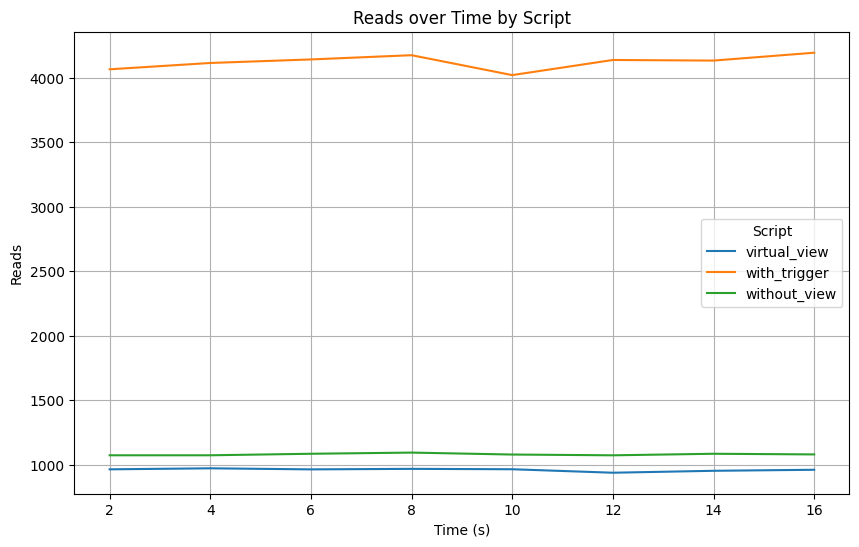
\includegraphics[width=\textwidth]{PNGs/Script/Views/view-comparison/Reads}
    \end{subfigure}
    \hfill
    \begin{subfigure}[t]{0.48\textwidth}
        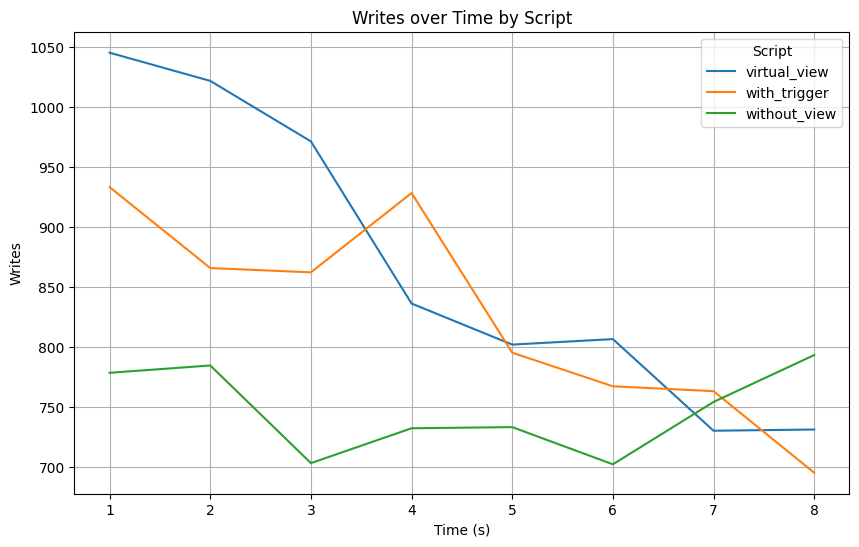
\includegraphics[width=\textwidth]{PNGs/Script/Views/view-comparison/Writes}
    \end{subfigure}
    \vspace{-5pt}
    \caption[Views: Keine View, virtuelle View und Ansatz mit Triggern]{Vergleich zwischen keiner View, der virtuellen und Triggeransatz in MySQL}
    \label{fig:view-comparison-comp-metric}
\end{figure}
\vspace{-15pt}

Bei den Ergebnissen fällt auf, dass die Unterschiede zwischen der virtuellen Sicht und den direkten SQL-Befehlen (\texttt{without\_view}) nur minimal sind.
Dennoch weist \texttt{with\_view} eine leicht schlechtere Performance auf, sowohl bei Lese- als auch bei Schreiboperationen (\ref{fig:view-comparison-comp-metric}).
Einen klaren Performancevorteil kann man beim Trigger-Ansatz erkennen, da die Lesewerte etwa um den Faktor 3 höher sind.
Das liegt daran, dass direkt die Tabelle mit den aggregierten Werten abgefragt wird, wodurch weniger Rechenaufwand erforderlich ist.
Anders hingegen sieht es bei der Schreibperformance aus, da die Trigger ausgelöst werden und zusätzliche Aktualisierungen an der Tabelle \texttt{KUNDEN\_MAT\_OVERVIEW} durchführt werden müssen.
Dadurch sehen wie einen deutlichen Unterschied zu den anderen beiden Ansätzen, da die Werte bei den Schreibvorgängen etwa 15--20\% langsamer sind.

Im letzten Benchmark sollen unterschiedliche Implementierungen von materialisierten Sichten getestet werden.
Dazu wird der Ansatz mit Triggern in MySQL mit der nativen Implementierung in PostgreSQL verglichen.
Die materialisierte Sicht in Postgres kann mithilfe des Befehls aus~\ref{lst:create_mat_view} direkt erstellt werden.
Da Postgres die inkrementeller Auffrischung nicht unterstützt, muss die materialisierte Sicht nach den \texttt{INSERT} und \texttt{DELETE}-Befehlen auf der Kundentabelle immer vollständig aktualisiert werden.
Da der Einfluss auf die Performance des Befehls~\ref{lst:refresh-materialized-view} untersucht werden soll, wird dieser einmal nach der Einfügung jeder Zeile in die Kundentabelle und einmal, nachdem alle Datensätze eingefügt wurden, ausgeführt.

Um die Performanceunterschiede zwischen PostgreSQL und MySQL zu ermitteln, wird der Trigger-Ansatz auch in PostgreSQL implementiert.
Die Implementierungen für die Insert- und Select-Befehle sind bei beiden DBMS identisch, bei der Erstellung der Tabellen und Trigger gibt es aber Unterschiede.
Zum einen unterscheiden sich die Mechanismen zur automatischen Generierung von Primärschlüsseln, da PostgreSQL \texttt{SERIAL} und MySQL \texttt{AUTO\_INCREMENT} verwendet.
Zum anderen kann in MySQL die Logik eines Triggers direkt in der \texttt{CREATE TRIGGER}-Anweisung definiert werden, während in PostgreSQL ein Trigger eine separate Funktion aufrufen muss, die die Logik enthält und mit \texttt{RETURNS TRIGGER} definiert ist.
Auch die Deklarierung der Variablen unterscheidet sich, da in PostgreSQL mehrere Variablen in einem \texttt{DECLARE}-Block und in MySQL jede Variable einzeln im \texttt{BEGIN...END}-Block deklariert werden muss.

\vspace{-5pt}
\begin{figure}[H]
    \centering
    \begin{subfigure}[t]{0.48\textwidth}
        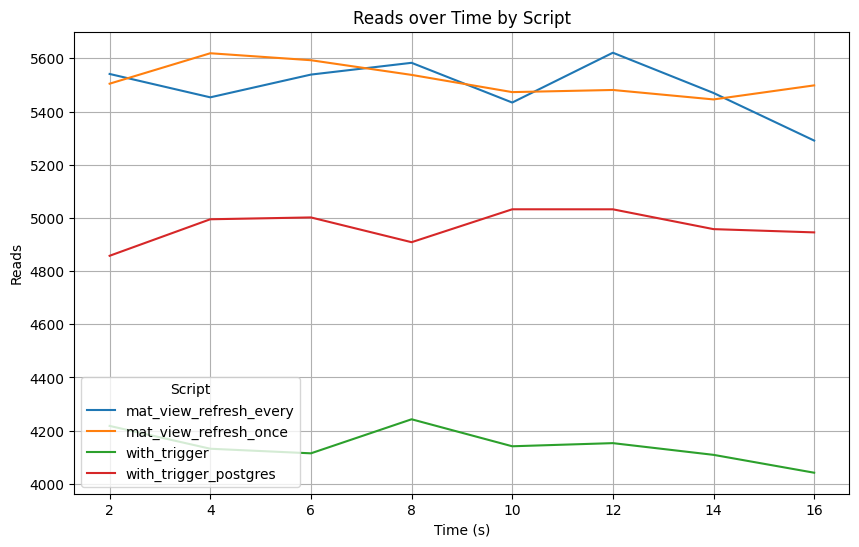
\includegraphics[width=\textwidth]{PNGs/Script/Views/mat-view-comparison//Reads}
    \end{subfigure}
    \hfill
    \begin{subfigure}[t]{0.48\textwidth}
        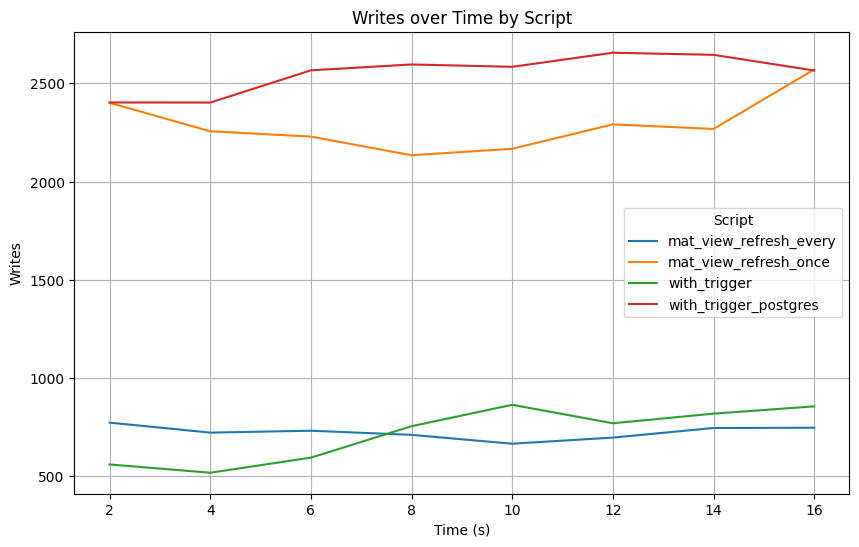
\includegraphics[width=\textwidth]{PNGs/Script/Views/mat-view-comparison/Writes}
    \end{subfigure}
    \vspace{-5pt}
    \caption[Views: Beide Triggeransätze sowie materialisierte Sicht]{Vergleich zwischen Triggeransatz in MySQL und Postgres, sowie zwei nativen Implementierungen in Postgres }
    \label{fig:mat-view-comparison-comp-metric}
\end{figure}
\vspace{-15pt}

Bei der Grafik~\ref{fig:mat-view-comparison-comp-metric} wird zuallererst ein sehr deutlicher Performanceunterschied beim Ansatz mit den Triggern zwischen PostgreSQL und MySQL sichtbar.
Begründet werden kann dieser Unterschied mit den verschiedenen Vorteilen des jeweiligen DBMS und dessen Umgebung.
Beide Systeme wurden mit dem gleichen Ansatz gebenchmarkt, um die Implementierung der nativen materialisierten Sicht, die nur in PostgreSQL möglich ist, besser vergleichen zu können.
Denn die Ergebnisse der nativen Implementierung sind in Bezug auf die Abfragegeschwindigkeit tatsächlich am performantesten und die Anzahl an Aktualisierungen (\ref{lst:refresh-materialized-view}) hat dabei keinen Einfluss.
Anders hingegen sieht es bei der Einfüge-Geschwindigkeit aus, da dort die Implementierung, die nach jedem Insert-Befehl aktualisiert nicht am schnellsten, sondern am langsamsten ist.
Der Vergleich zwischen den Datenbankmanagementsystemen fällt wieder schwer, da die Unterschiede zwischen \texttt{with\_trigger} und \texttt{with\_trigger\_postgres} sehr groß sind (etwa um Faktor 2--3).
Damit wird noch einmal deutlich wie stark die Einfügedauer bei den materialisierten Sichten von der Anzahl an Refreshs abhängig ist, da \texttt{mat\_view\_refresh\_every} unterhalb der Performance von \texttt{with\_trigger} liegt.
In vorliegenden Beispiel ist die einmalige Aktualisierung der Sicht besser als das Verwenden der Trigger in Postgres.

Es lässt sich also zusammenfassen, dass virtuelle Sichten wenig Auswirkungen auf die Performance haben.
Dies ist im eigentlichen Sinne aber auch nicht der Absicht der virtuellen Sicht, denn sie ist besser geeignet, um beispielsweise die Organisation der Rechte für unterschiedliche Nutzer der Datenbank zu gewährleisten.
Wenn man hingegen beispielweise in OLTP-Systemen die Notwendigkeit hat, dass man aggregierte Daten häufig zu der Analyse von bestimmten Daten benötigt, dann sind materialisierte Sichten nützlich.
Man sollte allerdings vor allem die Performanceauswirkungen von diesen Sichten nicht unterschätzen und sich gut überlegen, wie häufig und zu welcher Zeit die Daten aktualisiert werden müssen.